\documentclass[sigconf,table]{acmart}

\usepackage[utf8]{inputenc}
\usepackage{graphicx}
\usepackage{subfig}
\usepackage{xcolor}
\usepackage{amsmath,amssymb}
\usepackage{ifthen}
\usepackage{xspace}
% \usepackage{cite}

\usepackage{algorithm}
%\usepackage[noend]{algpseudocode}
\usepackage{algpseudocode}
\usepackage{color}
\usepackage{listings}
\usepackage{pifont}
\usepackage{multirow}
\usepackage{url}
%\usepackage{natbib}
%\usepackage[colorlinks=false,linkcolor=blue,urlcolor=blue,citecolor=blue,bookmarks=false,draft]{hyperref}
\renewcommand*{\UrlFont}{\ttfamily\rm}

\usepackage{listings}

\lstset{
  float,
  basicstyle       = \small\ttfamily,
  columns          = fixed,
  numbers          = left,
  numberstyle      = \tiny\ttfamily,
  numbersep        = 5pt,
  xleftmargin      = 5pt,
  xrightmargin     = 10pt,
  frame            = tb,
  captionpos       = b,
  upquote          = true,
  showstringspaces = false,
}

%\newcommand{\comment}[1]{}

% \usepackage{array}
% \usepackage{multirow}
% \usepackage{paralist}
% \usepackage{ragged2e}

% \usepackage[subtle]{savetrees}

% \usepackage[small,compact,noindentafter]{titlesec}
% \titlespacing\section{0pt}{6pt plus 2pt minus 2pt}{2pt plus 2pt minus 2pt}
% \titlespacing\subsection{0pt}{4pt plus 2pt minus 2pt}{2pt plus 1pt minus 1pt}
% \titlespacing{\paragraph}{0pt}{2pt plus 0pt minus 1pt}{1.0ex}

% \usepackage{setspace}
% \usepackage[margin=8pt,font={small,bf,stretch=0.85}]{caption}

% \usepackage{enumitem}
% \setitemize{noitemsep,topsep=3pt,parsep=3pt,partopsep=3pt}

% \usepackage[inline]{enumitem}
% \setlist{noitemsep,topsep=0pt,parsep=0pt,partopsep=0pt}

% \def\arraystretch{0.9}

\newcommand{\SYS}{\textsc{SecureStreams}\xspace}
\newcommand{\zmq}{\mbox{\textsc{ZeroMQ}}\xspace}
\newcommand{\rxl}{\mbox{\textsc{RxLua}}\xspace}
\newcommand{\luavm}{\mbox{\textsc{LuaVM}}\xspace}

\setlength{\textfloatsep}{10pt}

\newboolean{showcomments}
\setboolean{showcomments}{true}
\ifthenelse{\boolean{showcomments}}
{ \newcommand{\mynote}[3]{
   \fbox{\bfseries\sffamily\scriptsize#1}
   {\small$\blacktriangleright$\textsf{\emph{\color{#3}{#2}}}$\blacktriangleleft$}}}
{ \newcommand{\mynote}[3]{}}
\newcommand{\pf}[1]{\mynote{Pascal}{#1}{pink}}
\newcommand{\vs}[1]{\mynote{Valerio}{#1}{blue}}
\newcommand{\ah}[1]{\mynote{Aurelien}{#1}{red}}
\newcommand{\rp}[1]{\mynote{Rafael}{#1}{orange}}
\newcommand{\rr}[1]{\mynote{Romain}{#1}{green}}

\definecolor{darkgreen}{rgb}{0.3,0.5,0.3}
\definecolor{darkblue}{rgb}{0.3,0.3,0.5}
\definecolor{darkred}{rgb}{0.5,0.3,0.3}

\lstdefinelanguage{LUA}{
  sensitive=true,
  keywordstyle=[1]{\color{darkblue}\bfseries},
  keywordstyle=[2]{\color{darkgreen}\bfseries},
  morekeywords=[1]{and,break,do,else,elseif,end,for,function,if,in,local,
    nil,not,or,repeat,return,then,until,while,require,alias},% Official LUA keywords
  morekeywords=[2]{},% Your private keywords
  otherkeywords={.,=,~,*,>,:},
  morestring=[b]",
  stringstyle={\color{darkred}\itshape},
  breaklines=true,
  breakatwhitespace=true,
  linewidth=\columnwidth,
  comment=[l]{--},
  escapeinside={(*@}{@*)}
}

\lstdefinelanguage{YAML}{
  sensitive=true,
  keywordstyle=[1]{\color{darkblue}\bfseries},
  keywordstyle=[2]{\color{darkgreen}\bfseries},
  morekeywords=[1]{image, entrypoint, environment, devices, hostname},% Official LUA keywords
  morekeywords=[2]{},% Your private keywords
  otherkeywords={.,=,~,*,>,:},
  morestring=[b]",
  breaklines=true,
  breakatwhitespace=true,
  linewidth=\columnwidth,
  comment=[l]{--},
  escapeinside={(*@}{@*)}
}

% Copyright
% \setcopyright{none}
%\setcopyright{acmcopyright}
%\setcopyright{acmlicensed}
\setcopyright{rightsretained}
%\setcopyright{usgov}
%\setcopyright{usgovmixed}
%\setcopyright{cagov}
%\setcopyright{cagovmixed}



%Conference
\setcopyright{acmcopyright}
\acmDOI{http://dx.doi.org/10.1145/3093742.3093927}
\acmISBN{978-1-4503-5065-5/17/06}
\acmConference{DEBS '17}{June 19-23, 2017}{Barcelona, Spain}
\acmYear{2017}
\copyrightyear{2017}
\acmPrice{15.00}

\begin{document}

\title{\SYS: A Reactive Middleware Framework for Secure~Data~Stream~Processing}
\date{}

\author{Aur\'elien Havet}
\affiliation{%
  \institution{University of Neuchâtel}
  \city{Neuchâtel}
  \country{Switzerland}
}
\email{aurelien.havet@unine.ch}

\author{Rafael Pires}
\affiliation{%
  \institution{University of Neuchâtel}
  \city{Neuchâtel}
  \country{Switzerland}
}
\email{rafael.pires@unine.ch}

\author{Pascal Felber}
\affiliation{%
  \institution{University of Neuchâtel}
  \city{Neuchâtel}
  \country{Switzerland}
}
\email{pascal.felber@unine.ch}

\author{Marcelo Pasin}
\affiliation{%
  \institution{University of Neuchâtel}
  \city{Neuchâtel}
  \country{Switzerland}
}
\email{marcelo.pasin@unine.ch}

\author{Romain Rouvoy}
\affiliation{%
  \institution{Univ. Lille / Inria / IUF}
  \city{Lille}
  \country{France}
}
\email{romain.rouvoy@univ-lille.fr}

\author{Valerio Schiavoni}
\affiliation{%
  \institution{University of Neuchâtel}
  \city{Neuchâtel}
  \country{Switzerland}
}
\email{valerio.schiavoni@unine.ch}

% The default list of authors is too long for headers}
\renewcommand{\shortauthors}{A. Havet, R. Pires, P. Felber, M. Pasin, R. Rouvoy, V. Schiavoni}

% I don't know how useful are these settings, but CR instructions say "Inserting the following commands before your \begin{document} will improve the page layout"
\clubpenalty=10000
\widowpenalty=10000

\begin{abstract}
The growing adoption of distributed data processing frameworks in a wide diversity of application domains challenges end-to-end integration of properties like security, in particular when considering deployments in the context of large-scale clusters or multi-tenant Cloud infrastructures.

This paper therefore introduces \SYS{}, a reactive middleware framework to deploy and process secure streams at scale.
Its design combines the high-level reactive dataflow programming paradigm with Intel{\textregistered}'s low-level \emph{software guard extensions} (SGX) in order to guarantee privacy and integrity of the processed data.
The experimental results of \SYS{} are promising: while offering a fluent scripting language based on \textsc{Lua}, our middleware delivers high processing throughput, thus enabling developers to implement secure processing pipelines in just few lines of code.
\end{abstract}

\keywords{Middleware, security, SGX, stream processing}

\maketitle


\section{Introduction}r\label{sec:introduction}
\vs{recheck the storyline and reframe where needed. Maybe stress more the security aspect and how TEE can help}

The data deluge imposed by a world of ever-connected devices, like the \emph{Internet of Things} (IoT), has fostered the emergence of novel data analytics and processing technologies to cope with the typical \emph{volume}, \emph{velocity} and \emph{variety} properties that characterize the big data era.
In particular, to support the continuous flow of information gathered by millions of IoT devices, data streams have emerged as a suitable paradigm to process data at scale.
However, as some of these data streams may convey sensitive information, stream processing requires to support end-to-end security mechanisms in order to prevent third-parties to access restricted data.

% Data streams are more and more predominant in today's era of big data.
% In the world of all-connected and the \emph{Internet-of-Things} (IoT), on market places, or elsewhere, data is continuously produced and consumed by a large diversity of stakeholders.
%The latest estimates predict a total of \vs{fill} TB/s to be analyzed efficiently and securely within the next 10 years.
% In this context, data streams are expected to be processed with a native support for reliability, scalability and security properties.
This paper introduces \SYS{}, our initial work on a middleware framework for developing secure stream processing in the Cloud.
\SYS{} supports the implementation, deployment and execution of stream processing tasks in distributed settings, from large-scale clusters to multi-tenant Cloud infrastructures.
In particular, \SYS{} adopts of message-oriented~\cite{mom}, responsive, resilient-to-faults middleware design.
Finally, it scales horizontally and vertically seamlessly \rp{SGX is limited in memory usage, which weakens the claim of vertical scalability} \rr{I agree that vertical elasticity is hard to justify given the SGX constraints, unless we introduce a different kind of vertical scalability}.
%Its design This middleware is designed according to The Reactive Manifesto: it is responsive, resilient, elastic and message driven\cite{reactivemanifesto}.
Briefly, its design is inspired by the dataflow programming paradigm~\cite{uustalu_essence_2005}: the developer combines together several independent processing components (\emph{e.g.}, mappers, reducers, sinks, shufflers, joiners) to compose several processing pipes.
The framework integrates an abstraction of the required deployment infrastructure.
\SYS{} smoothly integrates with industrial-grade lightweight virtualization technologies (\emph{e.g.}, Docker~\cite{docker}).
%by deployment automation based on the Docker ecosystem
It aims to be secure: communication channels use the SSL protocol~\cite{freier2011secure} for data communication.
Finally, our design intends to exploit the secure processing capabilities offered by trusted hardware \emph{enclaves}, nowadays widely available into mass-market thanks to the introduction of Intel's \emph{Software Guard eXtensions} (SGX)~\cite{costan_intel} in the SkyLake processors~\cite{intel:skylake}, therefore offering end-to-end security to the processed streams.
% and giving the ability to process datas in trusted enclaves by the integration of the Intel's Software Guard Extension (SGX) hardware.

A few mainstream solutions exist today for distributed stream processing.
\textsc{Reactive Kafka}~\cite{reactivekafka} allows stream processing atop of Apache \textsc{Kafka}~\cite{apachekafka}.
More recently, few open-source solutions (\emph{e.g.}, Apache \textsc{Spark Streaming}~\cite{apachesparkstreaming}, Apache \textsc{Storm}~\cite{apachestorm}, \textsc{Infinispan}~\cite{infinispan}) introduced APIs to allow developers to quickly setup and deploy stream processing infrastructures.
These systems rely on the \emph{Java Virtual Machine} (JVM)~\cite{lindholm2014java}.
However, SGX currently imposes a hard memory limit of 128\,MB to the enclaved code and data, at the cost of expensive encrypted memory paging mechanisms and serious performance leaks~\cite{pires_scbr:2016,brenner_securekeeper:_2016} when this limit is crossed.
\SYS{} therefore proposes a lightweight and low-memory footprint framework that can fully execute within SGX enclaves.
We detail our implementation choices in Section~\ref{sec:implementation}.

%But one of our goals is to find out a software technology that can run in a SGX enclave, and the memory of the latter is limited to 96MB for the Intel Skylake processor (the first and only processor including SGX currently)\cite{costan_intel}.
%If the application running inside an enclave needs more memory, an expensive encrypted memory paging mechanism then is used, causing serious performance leaks~\cite{brenner_securekeeper:_2016}.
To recap, our \textbf{contributions} are the followings: (i) the design of \SYS{}, (ii) some details of our reference implementation, and (iii) the results of our preliminary evaluation based on a real-world dataset.

The remainder of this paper is organized as follows.
The architecture of \SYS{} is described in Section~\ref{sec:architecture}.
Our implementation choices and an example of \SYS{} program are reported in Section~\ref{sec:implementation}.
Section~\ref{sec:eval} discusses on our preliminary evaluation with respect to throughput and scalability results.
Before concluding, we wrap up by briefly describing our future work in Section~\ref{sec:future}.


\begin{figure}[!t]
  \centering
  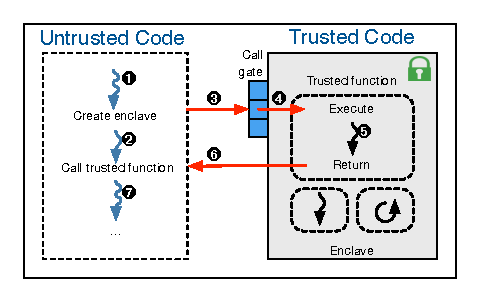
\includegraphics[scale=0.8]{images/sgx.pdf}
  \caption{SGX operating principles.}
  \label{fig:sgx}
\end{figure}

\section{SGX Lightning Tour}
\label{sec:background}
The design of \SYS revolves around the availability of SGX features in the host machines. 
It consists in a form of Trusted Execution Environment (TEE) recently introduced into Intel SkyLake, similar in the spirit to ARM TrustZone~\cite{arm2009security}. 
Applications create secure enclaves to protect the integrity and the confidentiality of the data and the code executed. 
The SGX mechanism, as depicted in Figure~\ref{fig:sgx}, allows applications to access confidential data from inside the enclave. 
The architecture guarantees that an attacker with physical access to a machine won’t be able to tamper with the application data. 
The CPU package represents the security boundary. 
Moreover, data belonging to an enclave is encrypted and authenticated when stored in main memory. 
A memory dump on a victim’s machine will produce encrypted data. 
A remote attestation protocol allows to verify that an enclave run on a genuine Intel processor with SGX. 
An application using enclaves must ship a signed (not encrypted) shared library (\emph{e.g.} a \texttt{.so} in Linux) that can possibly be inspected by malicious attackers. 
The Enclave Page Cache (EPC) is a 128 MB area of memory predefined at boot to store enclaved code and data. 
At most 90 MB can be used by application’s memory pages. 
Any access to an enclave page that dos not reside in the EPC triggers a page fault. 
The SGX driver interacts with the CPU to choose which pages to evict. 
The traffic between the CPU and the system memory is kept confidential by the memory encryption engine (MEE)~\cite{gueron2016memory}, also in charge of tamper resistance and replay protection. 
If a cache miss hits a protected region, the MEE encrypt or decrypt data before sending to, respectively fetching from, the system memory. 
Data can also persisted on stable storage protected by a seal key. 
This is useful in case the application restarts an enclave but without a new remote attestation.

The execution flow of a program using SGX enclaves is like the following.
First, an enclave is created (Figure~\ref{fig:sgx}-\ding{202}).
As soon as a program needs to execute a trusted function (Figure~\ref{fig:sgx}-\ding{203}), it executes SGX's \texttt{ecall} (Figure~\ref{fig:sgx}-\ding{204}).
The call goes through the SGX call gate to bring the execution flow inside the enclave (Figure~\ref{fig:sgx}-\ding{205}).
Once the trusted function is executed by one of the enclave's threads (Figure~\ref{fig:sgx}-\ding{206}), its result is encrypted and sent back the result (Figure~\ref{fig:sgx}-\ding{207}) before giving back the control to the main processing thread (Figure~\ref{fig:sgx}-\ding{208}).

\section{Architecture}\label{sec:architecture}

The architecture of \SYS{} comprises a combination of two different types of base components: \textsf{worker} and \textsf{router}.
A \textsf{worker} component continuously listens for incoming data by means of non-blocking I/O.
As soon as data flows in, an application-dependent business logic is applied.
A typical use-case is the deployment of a classic filter/map/reduce pattern from the functional programming paradigm~\cite{bird_introduction_1988}.
In such a case, worker nodes execute only one function, namely \texttt{map}, \texttt{filter}, or \texttt{reduce}.
A \textsf{router} component acts as a message broker between workers in the pipeline and transfers data between them according to a given \emph{dispatching policy}.
Figure~\ref{fig:architecture_pipeline} depicts a possible implementation of this dataflow pattern using the \SYS{} middleware.

\begin{figure*}[!t]
  \centering
  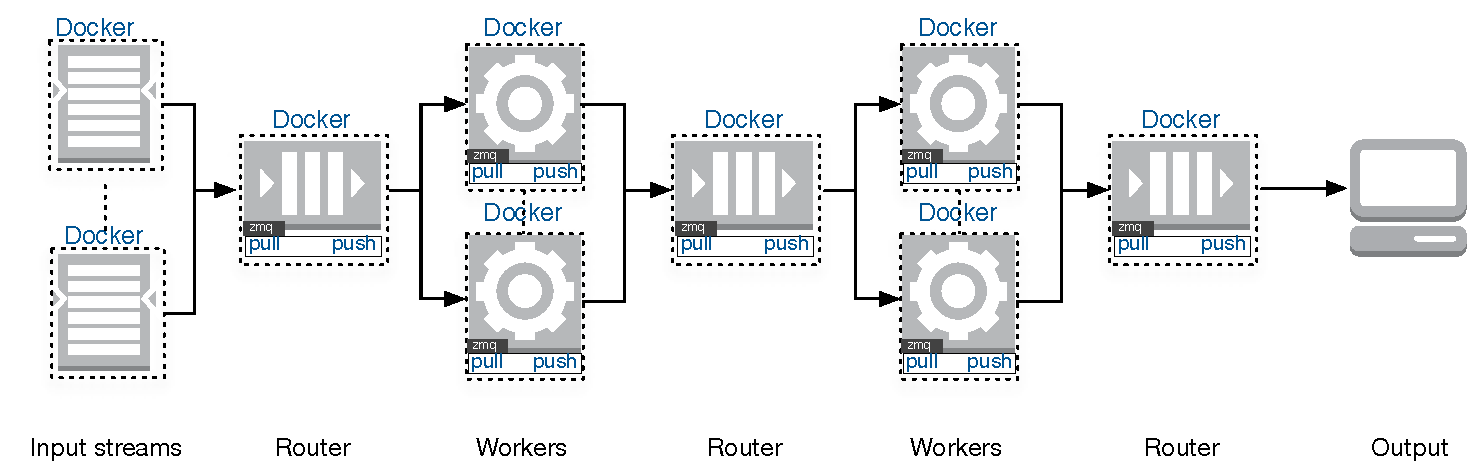
\includegraphics[width=\linewidth]{images/architecture_pipeline}
  \caption{Example of \SYS{} pipeline architecture.}
  \label{fig:architecture_pipeline}
\end{figure*}


\SYS{} is designed to support the processing of sensible data inside SGX enclaves.
As explained in the previous section, the \emph{enclave page cache} (EPC) is currently limited to $128\,MB$.\footnote{Future releases of SGX might relax this limitation~\cite{mckeen2016intel}.}
To overcome this limitation, we settled on a lightweight yet efficient embeddable runtime, based on the \textsc{Lua} virtual machine (\textsc{LuaVM})~\cite{ierusalimschy_luaextensible_1996} and the corresponding multi-paradigm scripting language~\cite{lualang}.
The \textsc{Lua} runtime requires only few kilobytes of memory, it is designed to be embeddable, and as such it represents an ideal candidate to execute in the limited space allowed by the EPC.
Moreover, the application-specific functions can be quickly prototyped in \textsc{Lua}, and even complex algorithms can be implemented with an almost 1:1 mapping from pseudo-code~\cite{leonini2009splay}.
We provide further implementation details of the embedding of the \textsc{LuaVM} inside an SGX enclave in Section~\ref{sec:implementation}.

%\rp{I would argue that the choice of Lua is not actually to overcome the memory limitation. I guess the majority of script interpreters would fit easily inside the 90MB. Besides, *ideal* is a quite strong claim. Of course we do need a script language since we cannot link code dinamically, but I would rather go with the programability arguments, the availability of RxLua, besides of course being easily embeddable and tiny.}

%If a process exceeds the available memory, an encrypted pagination mechanism leads to performance leaks.
%Thus \textsc{SecureStreams} has been designed to use a Lua runtime.
%Lua is a lightweight multi-paradigm programming language designed primarily for embedded systems and clients\cite{ierusalimschy_luaextensible_1996}.
%Its runtime requires only few KB of memory, and thus fits easily in EPC.

Each component is wrapped inside a lightweight Linux container (in our case, the \emph{de~facto} industrial standard Docker~\cite{docker}).
Each container embeds all the required dependencies, while guaranteeing the correctness of their configuration, within an isolated and reproducible execution environment.
By doing so, a \SYS{} processing pipeline can be easily deployed without changing the source code on different public or private infrastructures.
For instance, this will allow developers to deploy \SYS{} on Amazon EC2 container service~\cite{awsec2container}, where SkyLake-enabled instances will soon be made available~\cite{amazonskylake}, or similarly to Google compute engine~\cite{gceskylake}.
The deployment of the containers can be transparently executed on a single machine or a cluster, using a Docker network and the Docker Swarm scheduler~\cite{docker:swarm_2016}.
%\rp{Does Amazon offer machines with Skylake processors with EPC enabled?}
%\ah{It's planned: https://aws.amazon.com/fr/about-aws/whats-new/2016/11/coming-soon-amazon-ec2-c5-instances-the-next-generation-of-compute-optimized-instances/ but we don't know if SGX will be enabled. Google intends also: http://fortune.com/2017/02/24/google-intel-cloud-chip/. Do we have to cite there references?}

The communication between workers and routers leverages \zmq{}, a high-performance asynchronous messaging library~\cite{zero_mq}.
Each router component hosts inbound and outbound queues.
In particular, the routers use the \zmq's pipeline pattern~\cite{zero_mq:pipeline} with the \textsc{Push}-\textsc{Pull} socket types. 
%\rp{Is 'protocol' the best definition? I would rather call it a 'pattern'}\ah{It is, this is one of the different protocols of communication implemented in ZMQ, like explained in the target of the given pointer}\rp{The pointer does not mention protocol to refer to that. push/pull refers to the role of socket endpoints. It is not an agreement on format and content of exchanged messages, as a 'protocol' would be best understood by a common reader.}

The inbound queue is a \textsc{Pull} socket.
The messages are streamed from a set of anonymous\footnote{\emph{Anonymous} refers to a peer without any identity: the server socket ignore which worker sent the message.} \textsc{Push} peers (\emph{e.g.}, the upstream workers in the pipeline).
The inbound queue uses a fair-queuing scheduling to deliver the message to the upper layer.
Conversely, the outbound queue is a \textsc{Push} socket, sending messages using a round-robin algorithm to a set of anonymous \textsc{Pull} peers---\emph{e.g.}, the downstream workers.

% \vs{if there is time, it could be useful to have a drawing that zooms into this aspect of the architecture, not the full pipeline}
This design allows us to dynamically scale up and down each stage of the pipeline in order to adapt it to application's needs or the workload.
Finally, \zmq{} guarantees that the messages are delivered across each stage via reliable TCP channels.
%The pattern is mostly reliable insofar as it will not discard messages unless a node disconnects unexpectedly.
%This fire-and-forget messaging is a messsaging pattern in which we do not expect a direct response to the message, as opposed to request-response protocols\cite{voelter_patterns_2003}.
% The absence of response to a message provides some relevant performances.

We define the processing pipeline components and their chaining by means of Docker's Compose~\cite{docker:compose} description language.
Listing~\ref{pipeline-desc} reports on a snippet of the description used to deploy the architecture in Figure~\ref{fig:architecture_pipeline}.
Once the processing pipeline is defined, the containers must be deployed on the computing infrastructure.
We exploit the \texttt{constraint} placement mechanisms to enforce the Docker Swarm's scheduler in order to deploy workers requiring SGX capabilities into appropriate hosts.
In the example, an \texttt{sgx\_mapper} nodes is deployed on an SGX host by specifying \texttt{"constraint:type==sgx"} in the Compose description.

\begin{lstlisting}[language=YAML,caption={\SYS pipeline examples. Some attributes (\texttt{volume}, \texttt{networks}, \texttt{env\_file}) are omitted.},label=pipeline-desc][!t]
sgx_mapper:
  image: "${IMAGE_SGX}"
  entrypoint: ./start.sh sgx-mapper.lua
  environment:
    - TO=tcp://router_mapper_filter:5557
    - FROM=tcp://router_data_mapper:5556
    - "constraint:type==sgx"
  devices:
    - "/dev/isgx"

router_data_mapper:
  image: "${IMAGE}"
  hostname: router_data_mapper
  entrypoint: lua router.lua
  environment:
    - TO=tcp://*:5556
    - FROM=tcp://*:5555
    - "constraint:type==sgx"

data_stream:
  image: "${IMAGE}"
  entrypoint: lua data-stream.lua
  environment:
    - TO=tcp://router_data_mapper:5555
    - "constraint:type==sgx"
    - DATA_FILE=the_stream.csv
\end{lstlisting}

%\vs{Add some paragraphs to  detail how  the interaction with the SGX enclaves work in the context of \SYS}
%\vs{It should be useful to describe how the dataflow pipeline is mapped to the underlying cluster.}


\section{Implementation}
\label{sec:implementation}

% \begin{itemize}
%   \item Extension of the library RxLua
%   \item Why reactive?
%     \url{http://www.reactivemanifesto.org/}
%   \item ØMQ Lua bindings
%   \item ØMQ queues with push/pull protocol - Fire-and-forget messaging: a messsaging pattern in which we do not expect a direct response to the message, as opposed to request-response protocols
% \end{itemize}

%On September 2014 has been published the Reactive Manifesto\cite{reactivemanifesto}.
%This one attempts to define the principles to build systems more flexible, loosely-coupled and scalable.
%A \textit{reactive system} has to follow the four Reactive Principles:
%
%\begin{itemize}
%  \item Responsive: it is quick to react to all users in order to ensure a consistently positive user experience;
%  \item Elastic: it is easily upgraded on demand in order to ensure responsiveness under various load conditions;
%  \item Resilient: it applies proper design and architecture principles in order to ensure responsiveness;
%  \item Message-driven: it is based on a message-passing architecture to establish a boundary between components that ensures loose coupling, isolation and location transparency, e.g. event-driven, actor-based, or both of them.
%\end{itemize}
%
%The responsiveness of a system needs both elasticity and resiliency.
%Finally, a message-driven architecture is the foundation of elastic, resilient and responsive systems, as shown on figure \ref{fig:reactive-traits}.
%
%\begin{figure}[t!]
%  \centering
%  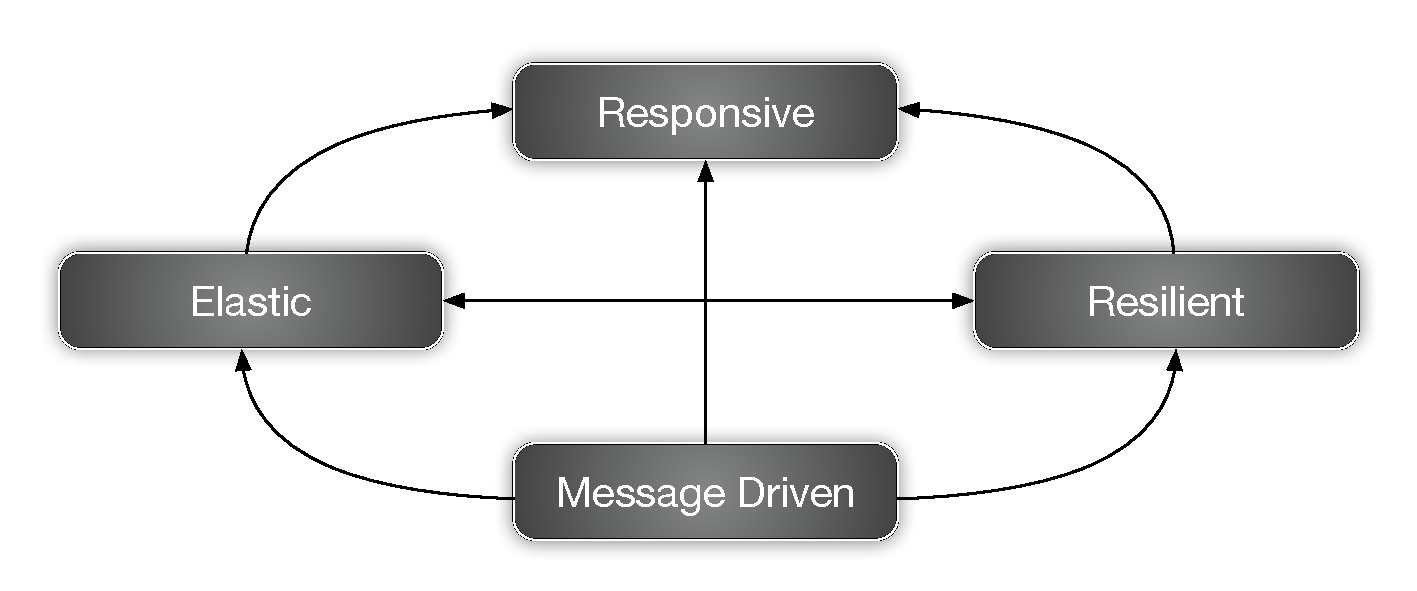
\includegraphics[width=.99\linewidth]{images/reactive-traits}
%  \caption{Reactive traits.}
%  \label{fig:reactive-traits}
%\end{figure}
%
%
%The term \textit{reactive} is not new in the field of computer sciences: Gérard Berry used it in 1989 while talking about \textit{real-time programming}\cite{berry:realtime_programming}.
%But recently the industry recognized the \textit{reactive paradigm} as the de facto way forward in system design\cite{malawski:why_reactive}.
%In the field of data streams, \textit{reactive programming} is programming with asynchronous streams, anything else.
%A stream is a sequence of ongoing events ordered in time, and these emitted events are captured only asynchronously by defining three functions:
%
%\begin{itemize}
%  \item an \textbf{onNext} function that will execute when a value is emitted;
%  \item an \textbf{onError} function executed when an error is emitted;
%  \item and finally an \textbf{onComplete} function executed when the stream is over.
%\end{itemize}
%
%
%
%A plenty of software libraries for different languages ensues from this paradigm\cite{reactive_streams}\cite{github:reactive_streams}.
%As exposed in section \ref{sec:architecture}, we chose the Lua technology as the basic of \SYS's implementation.
%Lua is a scripting language that is simple, efficient, extensible, functionnal and open-source\cite{ierusalimschy_programming_2006}.
%It will be easy to handle for the end user of \SYS.
%By the way, it is embedded in many application programs, such as Adobe Lighroom, Nmap, World of Warcraft or Nginx.


\SYS is implemented in Lua (v5.3).
Our implementation is compact, as it consists of only 120 lines of code (without counting the dependencies).
The framework partially extends \rxl~\cite{github:rxlua}, a library for reactive programming in Lua.
\rxl provides to the developer the required API to design a data stream processing pipeline following a dataflow programming pattern~\cite{uustalu_essence_2005}.
Listing~\ref{pipeline-example} shows an example of a \rxl program (and consequently, a \SYS{} program) to compute the average age of a population by chaining \texttt{:map}, \texttt{:filter} and \texttt{:reduce} functions.
The \texttt{:subscribe} function performs the subscription of 3 functions to the data stream.
These functions are observers, and the stream is an observable: this is precisely an implementation of the \textit{Observer Design Pattern}~\cite{szallies_using_1997}.
%A simple program example, computing from a source of \textit{people} the average age of the adult ones, throw a map/filter/reduce pipeline, is presented in listing \ref{pipeline-example}.

\SYS{} dynamically ships the business logic for each component into a dedicated Docker container and executes it.
%Our extension takes the business logic in each element of the pipeline to send and execute it in a Docker container.
The communication between the Docker container happens through \zmq (v4.1.2) and the corresponding Lua bindings~\cite{github:lzmq}.
%Then, the data is streamed accross the network communication built on top of the ØMQ protocol and implemented using the ØMQ Lua bindings\cite{github:lzmq}.
In summary, \SYS{} abstracts the underlying infrastructure from the developer, relying on \zmq and Docker.
We plan to release our code as open-source.

%\begin{minipage}{\linewidth}
\begin{lstlisting}[language=LUA,caption={Example of process pipeline with RxLua.},label=pipeline-example]
Rx.Observable.fromTable(people)
 :map(
   function(person)
     return person.age
   end
 )
 :filter(
   function(age)
     return age > 18
   end
 )
 :reduce(
   function(accumulator, age)
     accumulator[count] = (accumulator.count
       or 0) + 1
     accumulator[sum] = (accumulator.sum
       or 0) + age
     return accumulator
   end,
 )
 :subscribe(
   function(datas)
     print("Adult people average:",
       datas.sum / datas.count)
   end,
   function(err)
     print(err)
   end,
   function()
     print("Process complete!")
   end
 )
\end{lstlisting}
%\end{minipage}

Since the system software is not trusted in the SGX threat model, system calls are not allowed inside secure enclaves.
That makes porting legacy applications, like the Lua interpreter, more effortful.
We traced all calls made by the interpreter to the standard C library and replaced them by mock implementations that either mimic the real behavior or just do nothing.
That means that pieces of script code that is meant to run inside enclaves will not perform as they were supposed to if they work on files, network sockets or use any other input/output instruction.
Despite being a limitation, this approach also reinforces security. 
Since the framework safely handles the data movement and their provisioning to enclaves, the Lua script that is to run within SGX should not use files or sockets anyway.
Even if it does, that will be caught by the inocuous mock functions and make the attempt harmless.

Another constraint that comes with secure SGX enclaves is the impossibility of linking code dynamically. 
The reason is that the assurance that a given code is running inside a SGX-enabled processor is made through the measurement of its content at the event of enclave creation.
Based on that, further attestation mechanisms guarantee the enclave integrity, which ultimately allows them to receive sensitive information, such as the keys with which sensitive data will be thereafter exchanged. 
If additional code were allowed, that assurance would no longer hold, which would render the system exploitable by malicious attackers.
A direct consequence of such limitation is the unfeasibility of plugging Lua extensions in the traditional dynamic linking way. Every extension has to be statically compiled and packed with the enclave code. To ease the development of applications that rely on \SYS{}, we packed \emph{json} and \emph{csv} parsers within our enclaved interpreter.

\begin{figure}[t!]
  \centering
  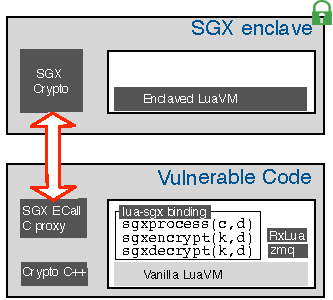
\includegraphics[scale=0.85]{images/arch-sgxlua.pdf}
  \caption{Integration between Lua and Intel SGX.}
  \label{fig:arch-luasgx}
\end{figure}


While this limited version of Lua was adapted to run inside SGX enclaves, we still needed to provide support for communication and the reactive streams framework itself.
That was done through a fully-fledged vanilla Lua interpreter, with a couple adaptations that allowed the interaction with the SGX enclaves.
Figure~\ref{fig:arch-luasgx} shows the conceived architecture.
The Lua interface was provided with 3 functions: \texttt{sgxprocess}, \texttt{sgxencrypt} and \texttt{sgxdecrypt}. The first forwars the encrypted code and data to be processed in the enclave while the others provide crypto functionalities.
In this work, we assume that attestation and key stablishment was previously done and we just happen to have a safe key inside the enclave.



\section{Evaluation}
\label{sec:eval}


This section reports on our evaluation of \SYS.
First, we present our evaluation settings.
Secondly, we detail the real-world dataset used in our experiments.
Finally, we analyze some preliminary benchmarks, namely throughput and scalability.


\textbf{Evaluation settings.}
We have experimented on machines using a processor Intel$^{\tiny{\textregistered}}$~Core\texttrademark~i7-6700~\cite{intel:i7_6700} and 8GB RAM.
We use a cluster of 2 machines based on Ubuntu 14.04.1 LTS (kernel 4.2.0-42-generic) and running a daemon Docker (v.1.13.0).
Machines are interconnected using a switched 1~Gbps network.
Nodes join a Docker Swarm cluster~\cite{docker:swarm_2016} (v1.2.5), using Consul~\cite{consul} (v0.5.2) as discovery service.
The Swarm manager and its discovery service are deployed on another machine.
Containers leverage the Docker overlay network to communicate to each other.

\vs{add SGX things}
\ah{in SGX things, explain the choice of Ubuntu 14.04.1}
\ah{should we reference public repositories and specific version (commit hashes) of used stuff (driver, platform) for SGX?}


\textbf{Dataset.}
In our experiments, we process a real dataset released by the \emph{American Bureau of Transportation Statistic}~\cite{rita:bts}.
The dataset reports on the flight departures and arrivals of 20 air carriers~\cite{statistical_computing:data}.
We implement a benchmark application atop of \SYS to compute average delays and the total of delayed flights for each air carrier.
We design and implement the full processing pipeline, that (i) parses the input datasets (in a comma-separated-value format) to data structure (\textsf{map}), (ii) filters data by relevancy (\emph{i.e.}, if the data concerns a delayed flight), and (iii) finally reduces it to compute the wanted informations.\footnote{This experiment is inspired by Kevin Webber's blog entry \emph{Diving into Akka Streams}: \url{https://blog.redelastic.com/diving-into-akka-streams-2770b3aeabb0}.}
We use the 4 last years of the available dataset (from 2005 to 2008), for a total of 28 millions of entries to process and 2.73 GB of data.
\vs{Update with the details of other datasets if any}
\ah{wouldn't it be more logical to puts Dataset section after Micro-Benchmark one?}


\textbf{Micro-Benchmark: Lua in SGX.}
\vs{NEW: here we show the overhead of executing Lua code inside/outside SGX enclaves. We should use well-known Lua benchmarks (maybe there are few in Lua's own test suite or come up with something that shows the trade-offs.)}
\vs{we should explore a bit the design space: how much data should be sent at once into the enclave before side-effects kick-in ? upon these results, we choose the proper parameter for the follow-up experiments.}

To estimate the cost of enclaved function calls we averaged the time it took to do one milion calls with no data transfers.
While normal function calls took 23.6 $ns$, enclaved calls took on average 2.35 $\mu s$, \textit{i.e}., two orders of magnitude worse.
We then assessed the cost of copying data from the unshielded execution to the enclave and compared with the time it took to natively do the same.
We initialized a buffer of 100 MB with random data and copied its content by chunks of increasing sizes, with one function call per chunk.
Figure~\ref{fig:sgxmemcpy} shows the results.
When using smaller chunks, the function call overhead plays an important role in the total time, which steadly drops until we send chunks of 64 KB (vertical line).
We can also notice that copying data back to non-sgx execution impose an overhead of at most 20\%.
Each point in the plot correspond to the average of 20 runs. Correctness of the copies was verified by SHA256 digest comparison between reproduced memory areas.

\begin{figure}[t!]
  \centering
  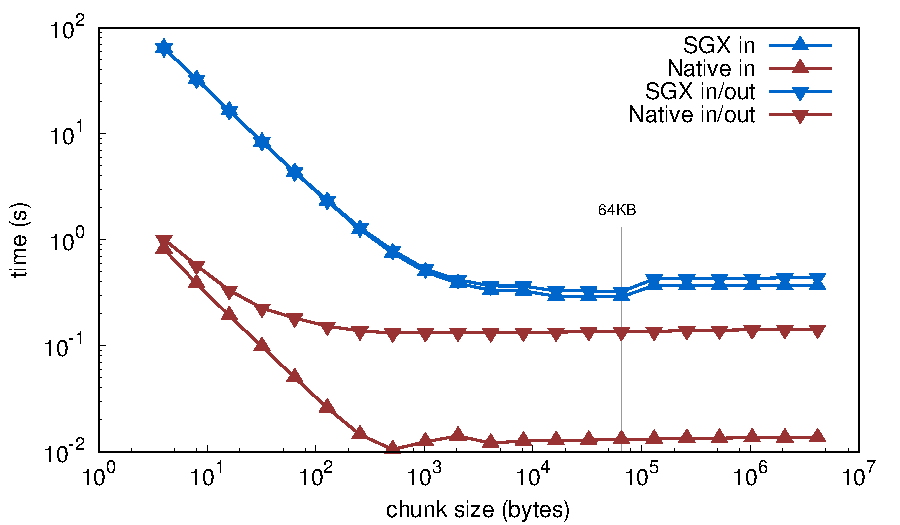
\includegraphics[scale=0.45]{plots/memcpy/memcpy.pdf}
  \caption{Time to copy 100 MB of memory}
  \label{fig:sgxmemcpy}
\end{figure}


Planned benchmarks:
\begin{itemize}
	\item overhead of the Lua benchmarks from \url{https://github.com/ltratt/vms_experiment/tree/master/benchmarks}
\end{itemize}
\textbf{Benchmark: throughput.}
This benchmark shows the upload throughput observed across the whole cluster while streaming the dataset as fast as possible from the source nodes into the processing pipeline.
We gather bandwidth measurements by exploiting Docker's own monitoring and statistical module.
%Throughput accross containers wrapping each node of the processing pipeline are measured from Docker stats.
The statistics are gathered at runtime while the experiment is executing.
%During the experiment, we retrieve all the data stats for each container.
%In particular, \texttt{txbytes} stats are extracted to measure containers output throughput.
We report on our results in Figure~\ref{fig:throughput}.
In this scenario, 4 nodes concurrently inject the input dataset into the processing pipeline, each one using a subset of the full dataset.
However, only one worker process is used for each step of the processing pipeline.
We use a representation based on stacked percentiles.
The white bar at the bottom represents the minimum value, the pale grey on top the maximal value.
Intermediate shades of grey represent the 25th, 50th–, median–, and 75th percentiles.
For instance, the median throughput at 200\,seconds into the experiment almost hits 2,500\,kB/s, meaning that 50\,\% of the nodes in that moment are outputting data at 2,500\,kB/s or less.
%These datas are computed to be plotted together by percentile, as shown on figure \ref{fig:throughput}.\ah{maybe it could be relevant to put three plots, corresponding to experiments 4-datas-1-worker, 4-datas-2-workers and 4-datas-4-workers}
With the current implementation, we observe a peak of 10\,MB/s upload throughput into the processing stages.%\vs{for the future, it'd be interesting to know which stage is the fastest one}
%\ah{I gonna measure throuput between two containers run on a swarm cluster, using iperf, for comparison purpose}


\begin{figure}[t!]
  \centering
  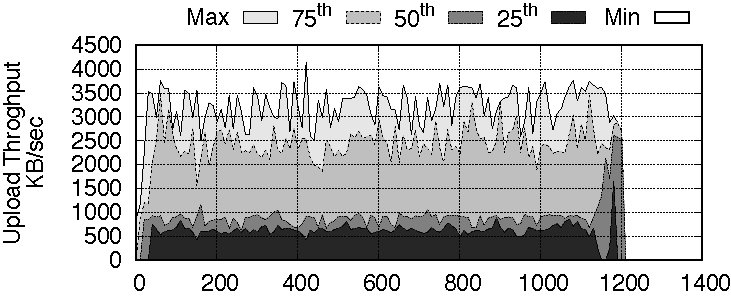
\includegraphics[scale=0.7]{images/tput_upload_4-datas-1-worker.pdf}
  \caption{Upload Throughput, single source. The middleware framework completes the processing of the dataset in 1,200\,seconds, with a peak of 4\,MB/s and an overall average throughput of 2.3\,MB/s}
  \label{fig:throughput}
\end{figure}

\vs{We should then extend this section to present how the TPUT is affected by having few/all streams going through the enclaves. This would be an interesting/useful plot as it provides useful insights.}


\textbf{Benchmark: scalability.} We conclude this preliminary by presenting scalability results of the \SYS framework.
In particular, we scale up each stage of the processing pipeline, up to 4\,workers per stage.
For each of the configurations, the experiment is repeated 20\,times.
We show average and standard deviation of the overall completion time to process the full dataset.
Figure~\ref{fig:scalability} depicts these results.
%Scalability of \SYS is evaluated by processing these datas 20 times on 3 different pipeline topology: using 1, 2 or 4 workers for each step of the pipeline.
We observe that by doubling the number of workers from the initial configuration achieves a 2$\times$ speed-up of the overall processing time, that is from 20\,minutes to less than 10\,minutes.
Conversely, we do not observe similar improvements when using 4\,workers.
%Results are represented on figure \ref{fig:scalability}, and show clearly better performances between the experiment using only one worker by task, and the one using 2 workers.
%In an other hand, using 4 workers instead of 2 does not show any performance improvement.

\begin{figure}[t!]
  \centering
  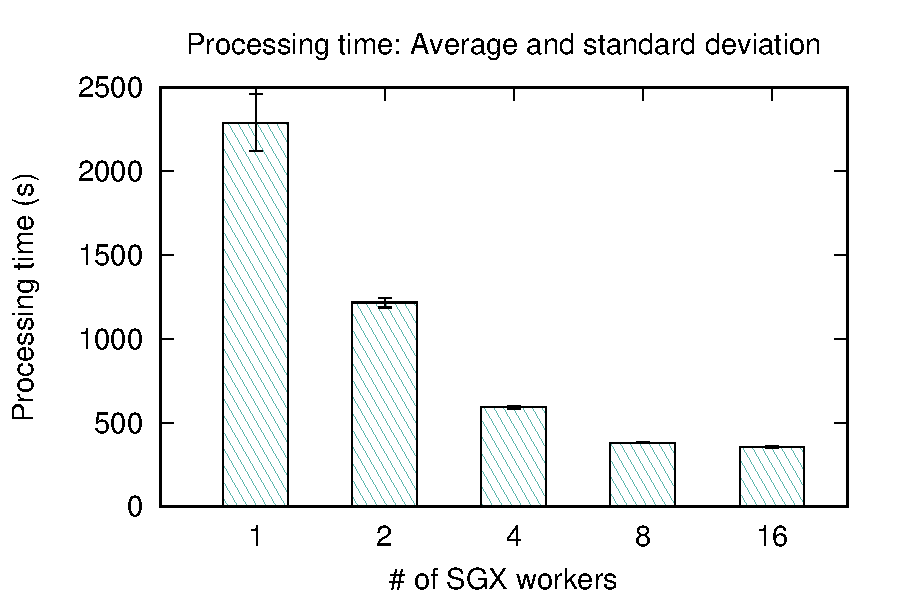
\includegraphics[scale=0.5]{plots/secure_streams/scalability/sgxmapper_scalability.pdf}
  \caption{Scalability: processing time, average and standard deviation. The experiment is repeated 5 times, with a variation on the number of mappers SGX, other workers do not use SGX.}
  \label{fig:scalability}
\end{figure}

We believe this behavior can be explained by existing bottlenecks in the pipelining infrastructure, lack of optimization in the application logic as well as tuning options of the \zmq queues.
These hypotheses are confirmed by observing the throughput of the system once we increase the processing workers to 2 and 4 in Figure~\ref{fig:throughput2} and Figure~\ref{fig:throughput4}, respectively.
We observe the following facts.
First, the system is far from saturating the network's available bandwidth, hitting a peak of 10\,MB/s.
Second, a small percentage of nodes consumes much more bandwidth than the other components.
We intend to further investigate these effects as part of our future work, as we are going to elaborate in the following section.

\begin{figure}[t!]
  \centering
  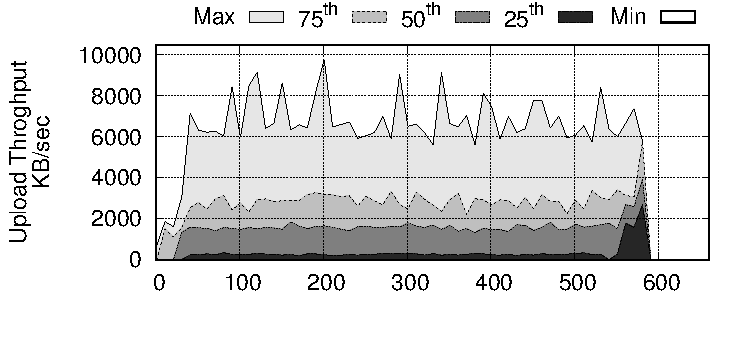
\includegraphics[scale=0.7]{images/tput_upload_4-datas-2-workers.pdf}
  \caption{Upload throughput, 2 concurrent processing workers by pipeline stage. Peak throughput at 10MB/s.}
  \label{fig:throughput2}
  \vspace{0.5cm}
  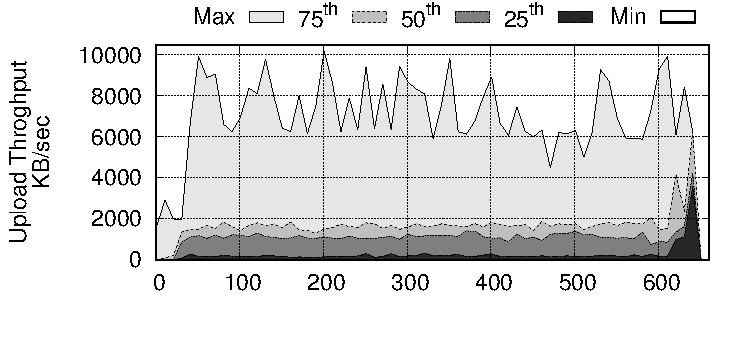
\includegraphics[scale=0.7]{images/tput_upload_4-datas-4-workers.pdf}
  \caption{Upload throughput, 4 concurrent processing workers by pipeline stage. Peak throughput at 10MB/s.}
  \label{fig:throughput4}
\end{figure}


\begin{figure*}[!t]
\centering
\begin{tabular}{cccc}
\subfloat[Throughput without encoding]{
  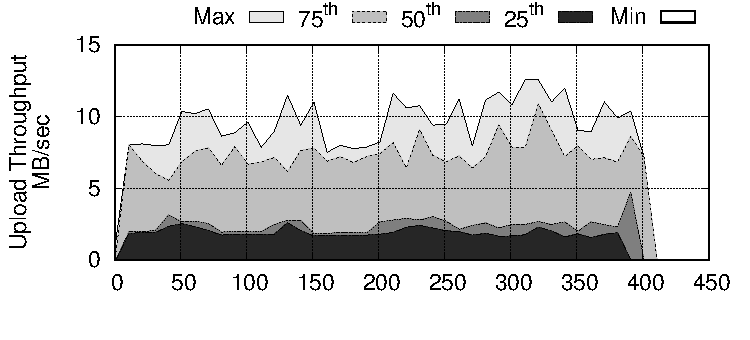
\includegraphics[width=.31\linewidth]{plots/secure_streams/throughput/tput_tx_percentiles_1-workers}
} &
\subfloat[Throughput without SGX]{
  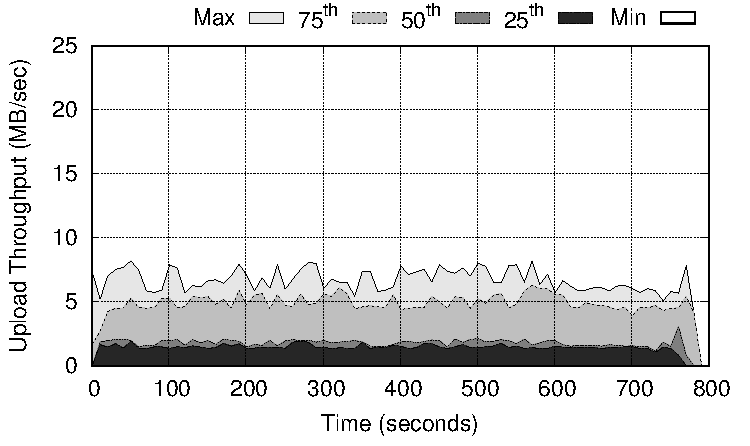
\includegraphics[width=.31\linewidth]{plots/secure_streams/throughput/tput_tx_percentiles_1-workers-encrypted-nosgx}
} &
\subfloat[Throughput with SGX]{
  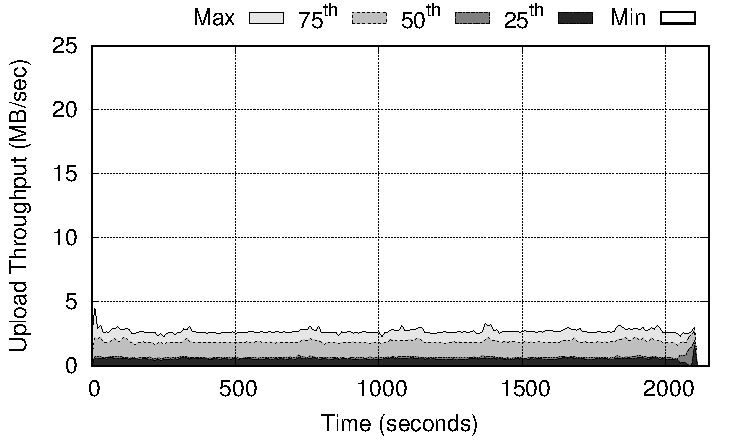
\includegraphics[width=.31\linewidth]{plots/secure_streams/throughput/tput_tx_percentiles_1-workers-encrypted-fullsgx}
}\cr
\subfloat[Throughput without encoding]{
  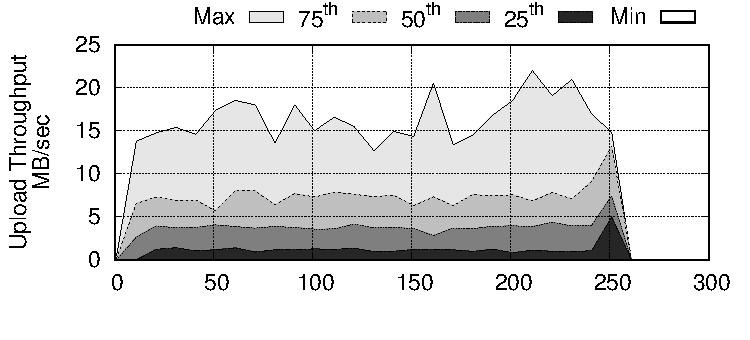
\includegraphics[width=.31\linewidth]{plots/secure_streams/throughput/tput_tx_percentiles_2-workers}
} &
\subfloat[Throughput without SGX]{
  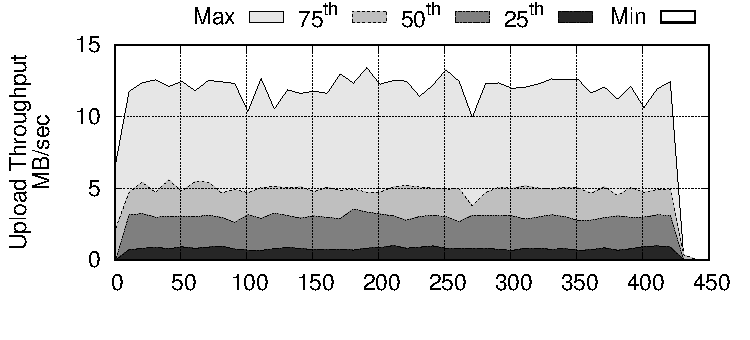
\includegraphics[width=.31\linewidth]{plots/secure_streams/throughput/tput_tx_percentiles_2-workers-encrypted-nosgx}
} &
\subfloat[Throughput with SGX]{
  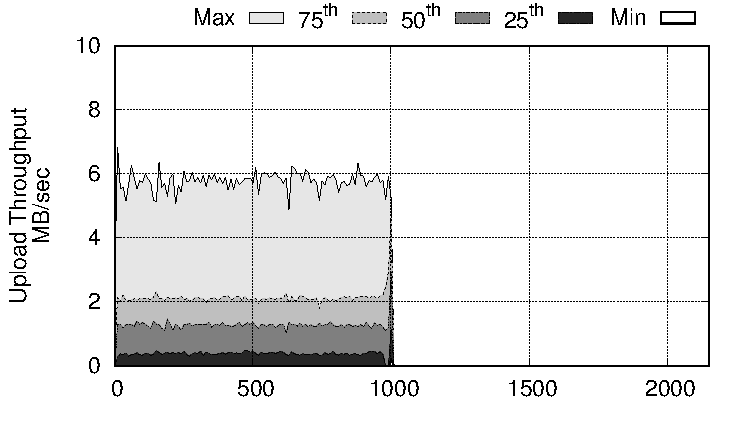
\includegraphics[width=.31\linewidth]{plots/secure_streams/throughput/tput_tx_percentiles_2-workers-encrypted-fullsgx}
}\cr
\subfloat[Throughput without encoding]{
  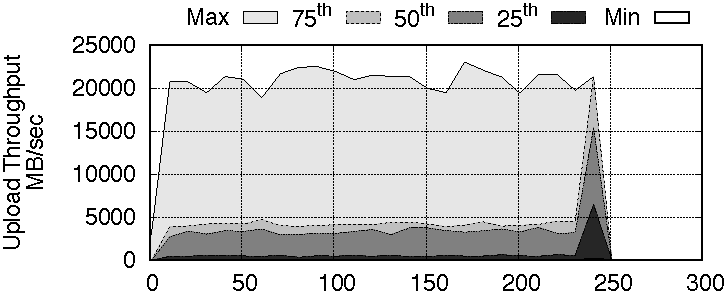
\includegraphics[width=.31\linewidth]{plots/secure_streams/throughput/tput_tx_percentiles_4-workers}
} &
\subfloat[Throughput without SGX]{
  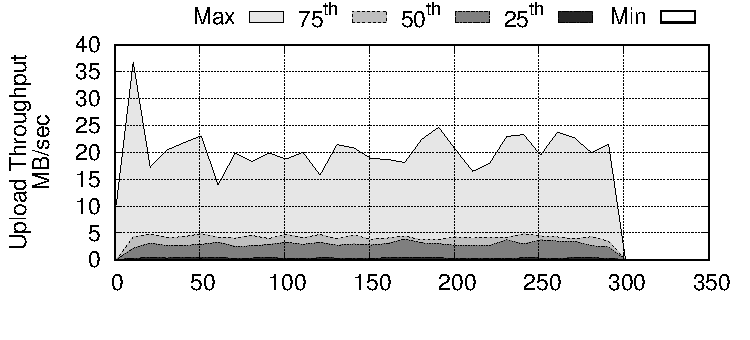
\includegraphics[width=.31\linewidth]{plots/secure_streams/throughput/tput_tx_percentiles_4-workers-encrypted-nosgx}
} &
\subfloat[Throughput with SGX]{
  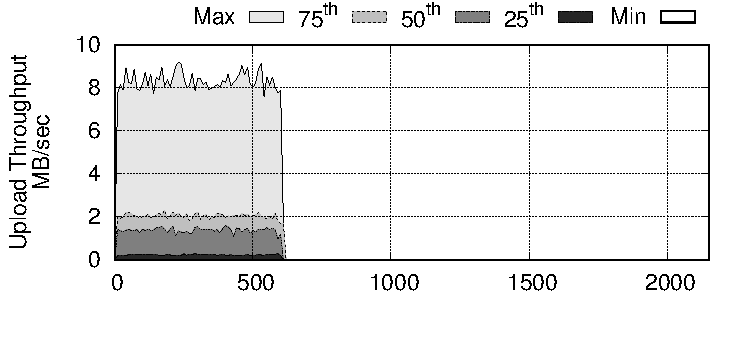
\includegraphics[width=.31\linewidth]{plots/secure_streams/throughput/tput_tx_percentiles_4-workers-encrypted-fullsgx}
}
\end{tabular}
\caption{Throughput comparison between normal processing and SGX processing}
\end{figure*}



\section{Related Work}\label{sec:rw}

%\vs{to do from scratch, should cover: stream processing papers, event-based middlewares, middleware that exploits hardware features}

Spark~\cite{Zaharia:2013:DSF:2517349.2522737} has recently gained a lot of traction as prominent solution to implement efficient stream processing.
It leverages Resilient Distributed Datasets (RDD) to provide a uniform view on the data to process.
Despite its popularity, Spark only handles unencrypted data and hence does not offer security guarantees.
Recent proposals~\cite{7840754} study possible software solutions to overcome this limitation.

Several big industrial players introduced their own stream processing solutions.
Thse systems are mainly used to ingest massive amounts of data and efficiently perform (real-time) analytics.
Twitter's Heron~\cite{Kulkarni:2015:THS:2723372.2742788}, and Google's Cloud DataFlow~\cite{Akidau:2015:DMP:2824032.2824076} are two prominent examples.
These systems are typically deployed on the provider's premises and are not offered \emph{as a service} to end-users.

A few dedicated solutions exist today for distributed stream processing using reactive programming.
For instance, \textsc{Reactive Kafka}~\cite{reactivekafka} allows stream processing atop of Apache \textsc{Kafka}~\cite{apachekafka,kreps2011kafka}.
These solutions do not, however, support secure execution in a trusted execution environment.

More recently, some open-source middleware frameworks (\emph{e.g.}, Apache \textsc{Spark}~\cite{apachesparkstreaming}, Apache \textsc{Storm}~\cite{apachestorm}, \textsc{Infinispan}~\cite{infinispan}) introduced APIs to allow developers to quickly set up and deploy stream processing infrastructures.
These systems rely on the \emph{Java} virtual machine (JVM)~\cite{lindholm2014java}.
However, SGX currently imposes a hard memory limit of 128\,MB to the enclaved code and data, at the cost of expensive encrypted memory paging mechanisms and serious performance overheads~\cite{pires_scbr:2016,brenner_securekeeper:_2016} when this limit is crossed.
Moreover, executing a fully-functional JVM inside an SGX enclave would currently consist in significant re-engineering efforts.

Few recent contributions tackle privacy-preserving data processing, particularly in a MapReduce scenario.
This is the case of Airavat~\cite{Roy:2010:ASP:1855711.1855731} and \textsc{Gupt}~\cite{Mohan:2012:GPP:2213836.2213876}.
These systems leverage differential-privacy techniques~\cite{dwork2006calibrating} and can face a different threat model than the one supported by SGX and hence by \SYS.
In particular, when deploying such systems on a public infrastructure, one needs to trust the cloud provider.
Our system greatly reduces the trust boundaries, and only require to trust Intel.

Some authors convene that public clouds may be secure enough some parts of an application.
They propose to split the jobs, running only the critical parts in private clouds.
A privacy-aware framework on hybrid clouds \cite{xu2015framework} has been proposed to work on tagged data, at different granularity levels.
A MapReduce preprocessor splits data into private and public clouds according to their sensitivity.
Sedic \cite{zhang2011sedic} does not offer the same tagging granularity, but proposes to automatically modify reducers to optimize the data transfers in a hybrid cloud.
These solutions require splitting application and data in two parts (sensitive and not) and impose higher latencies due to data transfers between two different clouds.
Yet, they cannot offer better security guarantees that the software stack itself offers, be it public or private.

MrCrypt \cite{tetali2013mrcrypt} proposes using homomorphic encryption instead of trusted elements.
Through static code analysis, it pinpoints different homomorphic encryption schemes for every data column.
Still, some of the demonstrated benchmarks are ten times slower than the unecrypted execution.
\SYS{} avoids of complex encryption schemes, decrypts data entering enclaves and processes in plaintext.

To best of our knowledge, \SYS{} is the first lightweight and low-memory footprint stream processing framework that can fully execute within SGX enclaves.


\section{Conclusion}
\label{sec:conclusion}

Secure stream processing is becoming a major concern in the era of the Internet of Things and big data.
This paper introduces our design and evaluation of \SYS{}, an concise and efficient middleware framework to implement, deploy and evaluate secure stream processing pipelines for continuous data streams.
The framework is designed to exploit the SGX \emph{trusted execution environments} readily available in Intel{\textregistered}'s commodity processors, such as the latest SkyLake.
We implemented the prototype of \SYS{} in \textsc{Lua} and based its APIs on the reactive programming approach.
Our initial evaluation results based on real-world traces are encouraging, and pave the way for deployment of stream processing systems over sensitive data on untrusted public clouds.

We plan to further extend and thoroughly evaluate \SYS in our future work.
In particular, we plan to extend \SYS with full automation of container deployments, as well as enriching the framework with a library of standard stream processing operators and efficient yet secure native plugins, to ease the development of complex stream processing pipelines.
\newpage



\section*{Acknowledgments}
The research leading to these results has received funding from the European Commission, Information and Communication Technologies, H2020-ICT-2015 under grant agreement number 690111 (SecureCloud project).
Rafael Pires is also sponsored by CNPq, National Counsel of Technological and Scientific Development, Brazil.

{
%\footnotesize
\bibliographystyle{ACM-Reference-Format}
\bibliography{biblio}
% \balancing
}

\end{document}
